\documentclass{article}
\usepackage{authblk}
\renewcommand{\thefigure}{S\arabic{figure}}

\title{NPDR Supplementary Material}
\author[1]{Trang T. Le}
\author[2]{Bryan A. Dawkins}
\author[2,3*]{Brett A. McKinney}
\affil[1]{Department of Biostatistics, Epidemiology and Informatics,
University of Pennsylvania, Philadelphia, PA 19104}
\affil[2]{Department of Mathematics, University of Tulsa, Tulsa, OK 74104}
\affil[3]{Tandy School of Computer Science, University of Tulsa, Tulsa, OK 74104}
\renewcommand{\Authands}{ and }

\usepackage{Sweave}
\begin{document}
\Sconcordance{concordance:sup_npdr.tex:sup_npdr.Rnw:%
1 14 1 1 0 20 1}

\setkeys{Gin}{width=1\textwidth}
\maketitle
\newpage
% \section{Performance comparison between NPDR and Relief-F}



% \begin{figure}[h]%figure1
% \centerline{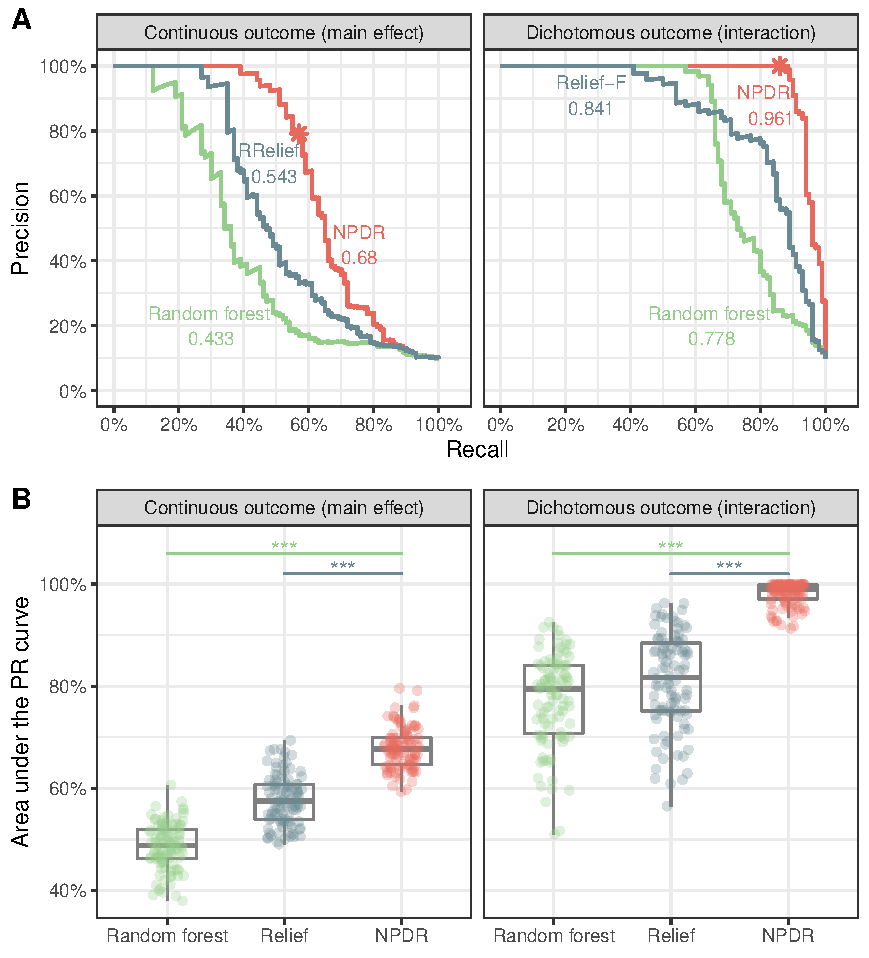
\includegraphics[]{../figs/pr_compare_100.pdf}}
% \caption{\textbf{Relief, NPDR and random forest comparison of area under the PRC (auPRC)} for 100 replicate simulations of continuous outcome data with main effect (left) and dichotomous outcome data with interaction effect (right). All simulations use $m = 200$ samples and $p = 1,000$ attributes with 100 functional. NPDR yields significantly higher auPRC in both simulation types.}
% \label{fig:auPRC}
% \end{figure}

\begin{figure}[h]%figure3
\centerline{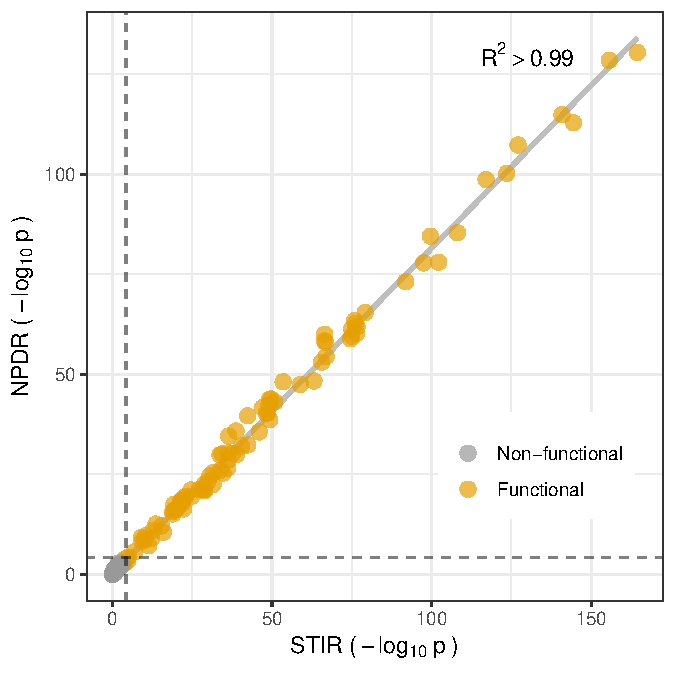
\includegraphics[]{../figs/npdr_stir_p_cc.pdf}}
\caption{\textbf{Similarity between NPDR and STIR (dichotomous outcomes).} Comparison of -log$_{10}$ P values for one interaction simulation of $m = 200$ (100 cases and 100 controls) and $p = 1000$ attributes with 100 functional. In 100 replicate simulations, correlation,  $r$, between the two methods ranges from 0.9827 to 0.9994. STIR is based on a t-test of projected distances and NPDR is based on a logistic regression of projected distances. NPDR has the added benefit of handling continuous outcomes and covariate correction.}
\label{fig:npdr_stir}
\end{figure}


\begin{figure}[h]%figure2
\centerline{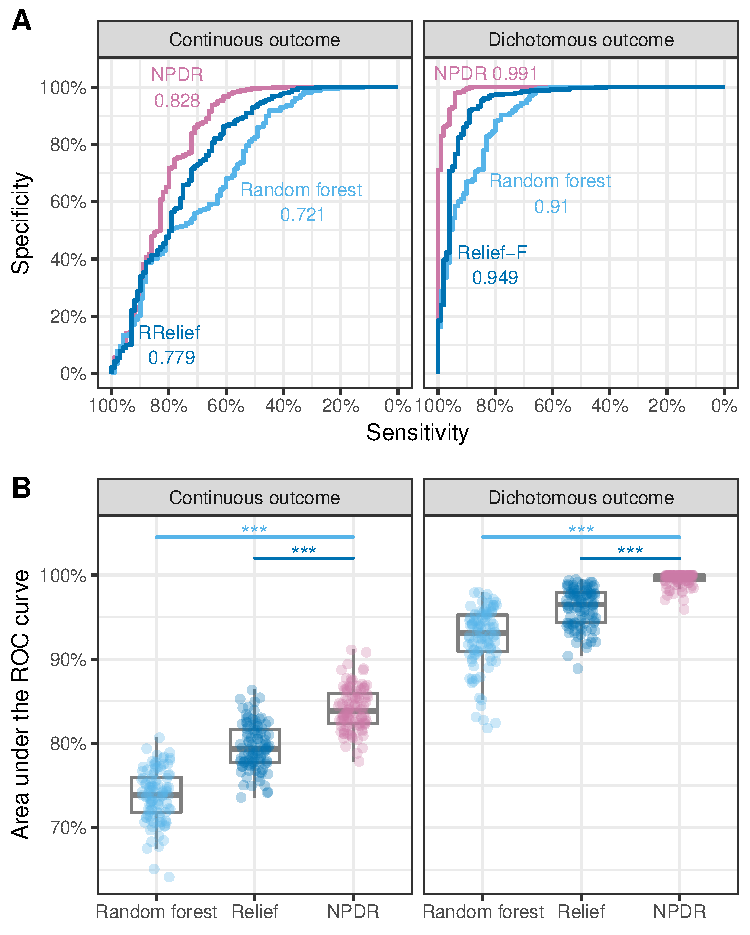
\includegraphics[]{../figs/roc_compare_100.pdf}}
\caption{\textbf{Receiver Operating Characteristic (ROC) curves for Relief, NPDR and random forest feature selection.} For one replicate simulation (A), ROCs for continuous outcome data with main effects (left) and dichotomous outcome data with interaction effects (right). The auROC value is given for each method. For 100 replicate simulations of both simulation types (B), NPDR yields statistically significant higher auROC than Relief or random forest ($\ast$$\ast$$\ast$ indicate P $<.0001$). All simulations use $m = 200$ samples and $p = 1,000$ attributes with 100 functional.}
\label{fig:auROC}
\end{figure}


% \begin{figure}[h]%figure
% \centerline{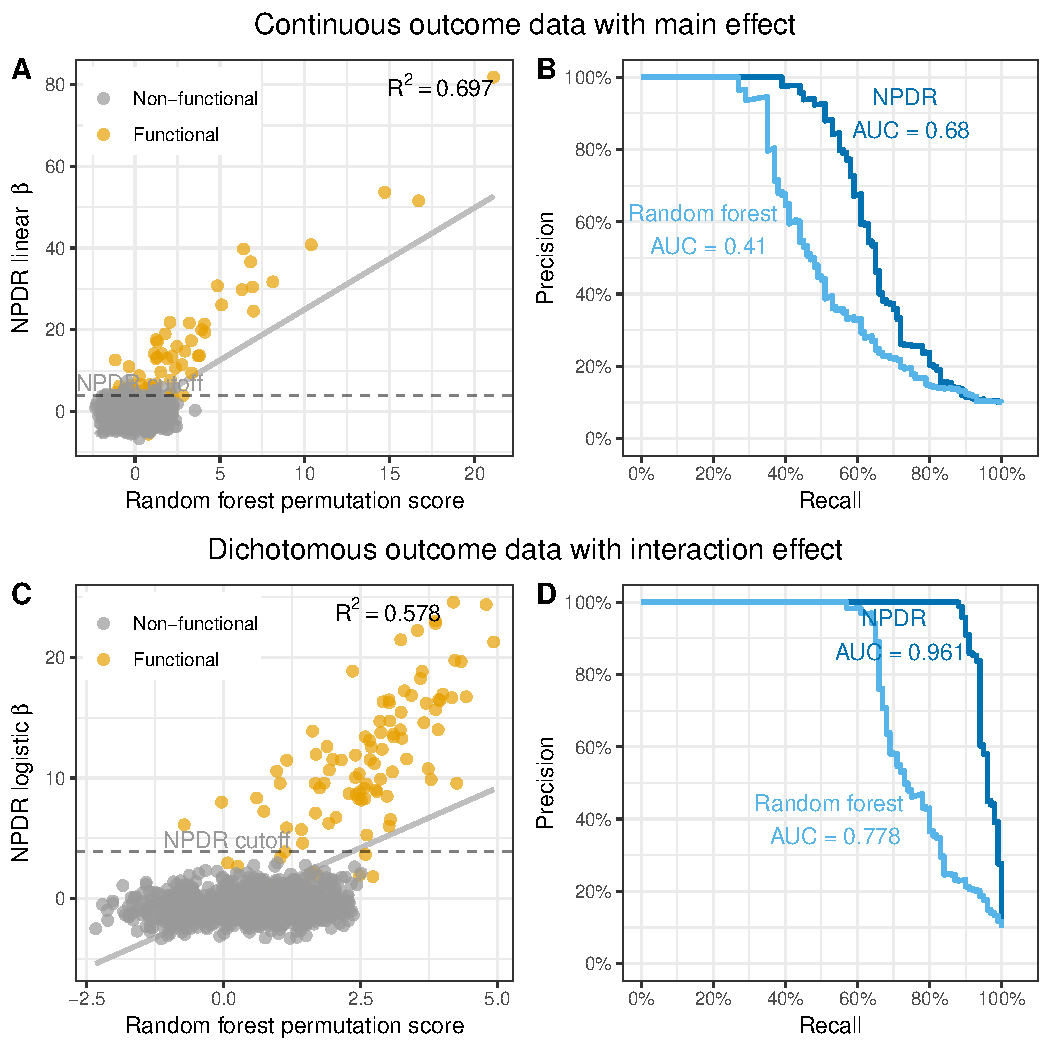
\includegraphics[]{../figs/npdr_rf.pdf}}
% \caption{\textbf{Comparison of NPDR and random forest importance scores} for continuous outcome data with main effects (top row) and dichotomous outcome data with interaction effects (bottom row). Results for one replicate simulation ($m = 200$ samples and $p = 1,000$ attributes with 100 functional). For continuous outcome (A), importance scores computed by random forest permutation (percent increase in MSE) and NPDR standardized linear regression coefficient. For case-control outcome (C), scores computed by random forest permutation (mean decrease in accuracy) and NPDR standardized logistic regression coefficient. A regression line between the scores with $R^2$ is shown, and a 0.05 Bonferroni cutoff (dashed) is shown for NPDR (A and C). There is no statistical threshold for random forest, so area under the precision-recall curve (auPRC) is used to compare algorithm performance (B, D).}
% \label{fig:auPRC}
% \end{figure}


% \begin{figure}[!tpb]%figure2
% \centerline{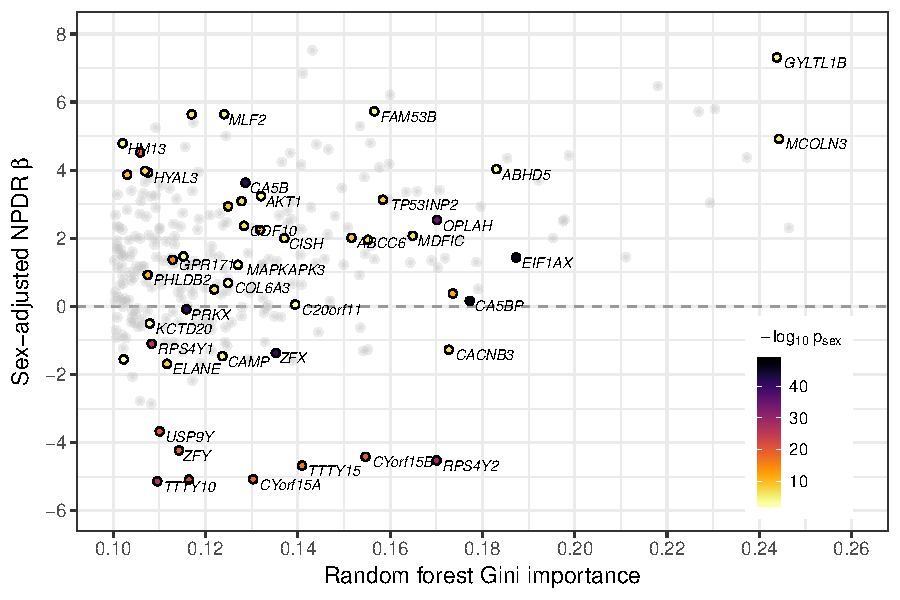
\includegraphics[]{../figs/mostafavi_npdr_rf_mdd.pdf}}
% \caption{{\bf NPDR vs random forest feature importance.}
% Gene scatter plot of importance score for association with major depressive disorder using random forest and NPDR with correction for sex. Most genes highly associated with sex are removed by adjustment in NPDR (above horizontal dashed line). Many genes with high random forest importance score also have high association with sex (dark genes). Top 50 genes with strongest association with sex are labeled. Alternatively, the \texttt{ranger} \texttt{R} package allows the option of forcing the inclusion of covariates (e.g., sex) in the model in addition to a set number of random variables selected prior to node splitting. However, when the forced covariate is associated with the outcome (potential confounding), the covariate has very high importance at the cost of diminished importance of other variables. In the case of the current real RNASeq data analysis of MDD, when we utilized this option in \texttt{ranger}, the covariate ``sex" is more than 20 times more important than the next most important attribute (ZNF845). To summarize, the effect of forced inclusion of a particular covariate at node splitting on the entire algorithm is unclear. More specific studies with simulations of covariates will prove useful in determining the effect of this implementation on the final result.}
% \label{fig:mostafavi_npdr_rf_mdd}
% \end{figure}

\begin{figure}[h]%figure
\centerline{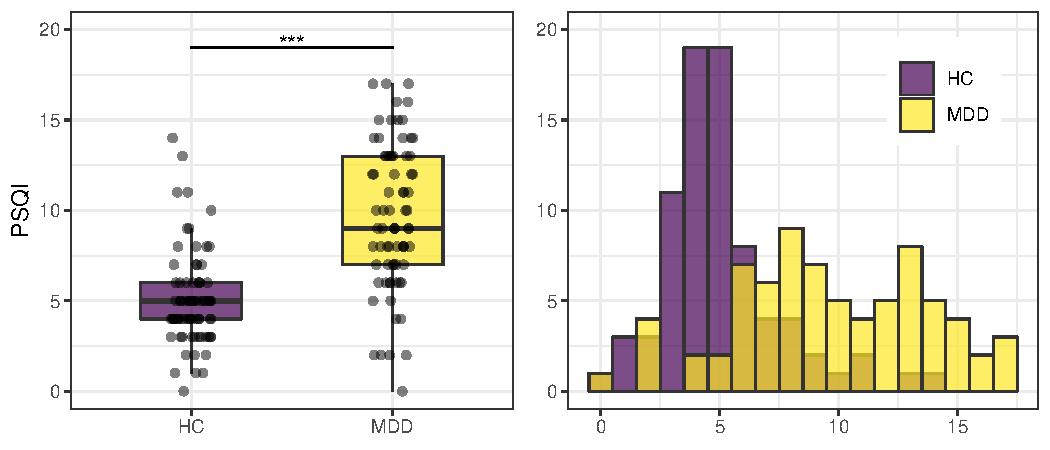
\includegraphics[]{../figs/psqi_plots.pdf}}
\caption{\textbf{The distribution of the Pittsburgh Sleep Quality Index (PSQI)} among individuals with and without MDD in Le et al.'s RNASeq dataset \cite{le18}.}
\label{fig:psqi_plots}
\end{figure}


\begin{figure}[h]%figure
\centerline{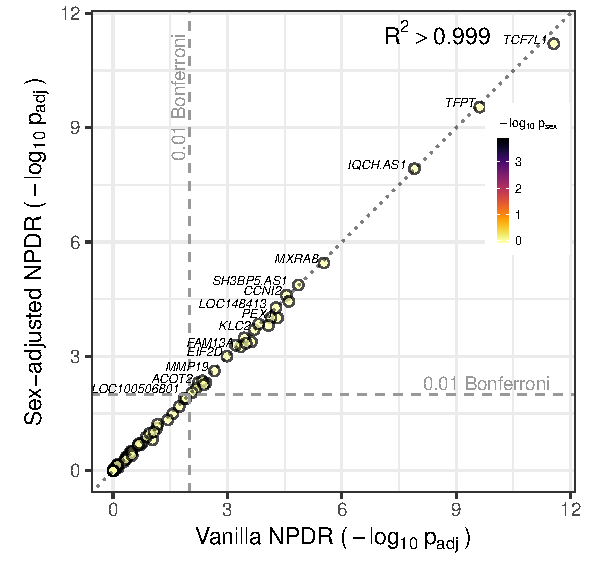
\includegraphics[]{../figs/jerzy_npdrs_mdd.pdf}}
\caption{\textbf{NPDR with and without sex adjustment for analysis of MDD-associated genes} in Le et al.'s RNASeq dataset \cite{le18}. Adjustment for the sex covariate has a negligible effect on the resulting P values for each important gene because of the balanced study design. Both methods yield consistent results with STIR from previous study (Fig. 4 of Ref. \cite{stir}), not shown.}
\label{fig:jerzy_npdrs_mdd}
\end{figure}

\clearpage
\bibliographystyle{unsrt}
\bibliography{NPDR_refs}   % name of bib file

\end{document}
